\section{Results}
\label{sec:results}

\Cref{tab:main} summarizes the estimates for the primary outcome from the three designs. The synthetic control is the primary causal specification; the international difference-in-differences and the regression discontinuity in time are complementary analyses of the same shock. The subsections below present each design's main figure and table.

% Generated by analysis/tables/make_all_tables.py -- do not edit by hand.
\begin{table}[htbp]
\centering
\footnotesize
\caption{Summary of estimates across designs: daily active-user rate}
\label{tab:main}
\begin{threeparttable}
\begin{tabular}{lrrrr>{\raggedright\arraybackslash}p{3.4cm}}
\toprule
Specification & Actual & Counter- & ATT & Relative & Diagnostic \\
 & BD (\%) & factual (\%) & (pp) & effect &  \\
\midrule
Synthetic control & 2.021 & 15.277 & $-$13.256 & $-$86.8\% & Pre RMSPE 3.260; ratio 4.192 \\
International DiD & 2.021 & 15.109 & $-$13.088 & $-$86.6\% & All donor countries \\
International DiD, no holidays & 2.021 & 15.400 & $-$13.379 & $-$86.9\% & National holidays excluded \\
RDiT, local linear & -- & -- & $-$9.284 & -- & HAC SE 5.034 pp; $p=0.065$ \\
\bottomrule
\end{tabular}
\begin{tablenotes}[flushleft]
\footnotesize\raggedright
\item \textit{Notes:} The outcome is the daily percentage of eligible users with observable productive GitHub activity; effects are averages over July 18--23, 2024. SC placebo rank values are $1/15=0.0667$ for both the absolute-ATT and RMSPE-ratio tests, the minimum attainable with 14 placebo countries (\cref{tab:sc_placebos}). The RDiT row is the preferred specification (cutoff July 17, bandwidth 7 days, degree 1, no donut, $N=15$ days, HAC lags 2) and is treated as a temporal robustness check, not as the main design.
\end{tablenotes}
\end{threeparttable}
\end{table}


\subsection{Synthetic control: main effect on daily productive activity}
\label{sec:main_results}

The synthetic-control estimate shows an exceptionally large collapse in observable GitHub activity (\cref{fig:sc,tab:sc_main}). Bangladesh's active-user rate averages 2.021 percent during July 18--23, compared with a synthetic counterfactual of 15.277 percent. The ATT is $-$13.256 percentage points, equivalent to an 86.8 percent reduction relative to the synthetic counterfactual. The pre-treatment RMSPE is 3.260 percentage points and the post/pre RMSPE ratio is 4.192.

\begin{figure}[htbp]
\centering
\caption{Actual and synthetic Bangladesh: daily share of eligible users with observable productive GitHub activity}
\label{fig:sc}
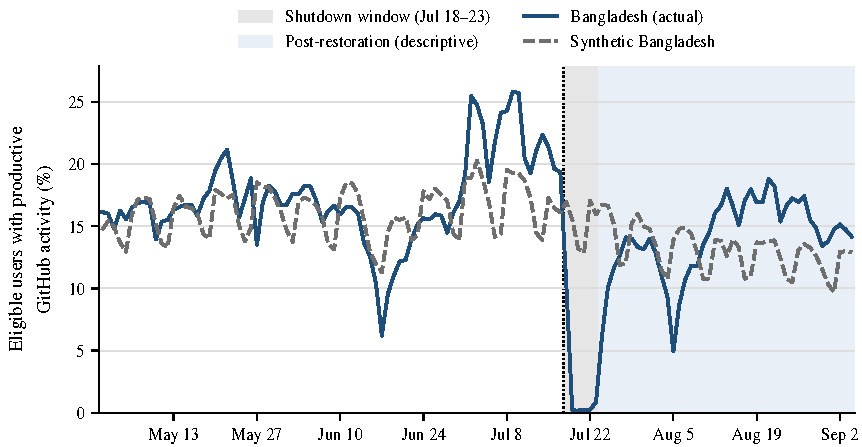
\includegraphics[width=\textwidth]{fig1_sc_actual_vs_synthetic.pdf}
\fignote{The solid line is the daily percentage of eligible Bangladesh-associated GitHub accounts with observable productive GitHub activity; the dashed line is the synthetic control, a weighted combination of Pakistan (47.6\%), Ghana (32.5\%), and Kenya (19.9\%) with weights chosen on May 1--July 17, 2024 (\cref{tab:sc_main}). The shaded shutdown interval defines the primary treatment estimand. Post-restoration differences are shown descriptively and are not interpreted as additional causal treatment effects. The grey band marks the July 18--23 shutdown and the dotted line its onset; the blue band marks the post-restoration period, July 24--September 4, over which the synthetic series is extended with the same weights. Average weekly gaps in weeks $+4$ and $+5$ after the shutdown (4.24 and 4.67 percentage points) remain within the range of pre-treatment weekly gaps ($-$2.86 to 5.88 percentage points). The dips on June 17 and August 5 coincide with national holidays coded in the country-day panel. Pre-treatment fit is imperfect (pre-treatment RMSPE 3.26 percentage points), most visibly in early July, when Bangladesh lies above its synthetic counterpart. The outcome measures observable public GitHub activity, not total software productivity. Sources: \texttt{results/synthetic\_control/actual\_vs\_synthetic\_daily.csv} (through July 23); \texttt{results/synthetic\_control/reproduced/sc\_daily\_path\_full.csv} and \texttt{sc\_weekly\_gaps.csv}, computed by \texttt{analysis/synthetic\_control/01\_reproduce\_sc.py}, which reproduces the archived weights and daily series exactly.}
\end{figure}

% Generated by analysis/tables/make_all_tables.py -- do not edit by hand.
\begin{table}[htbp]
\centering
\small
\caption{Synthetic control: main estimates and placebo inference}
\label{tab:sc_main}
\begin{threeparttable}
\begin{tabular*}{0.72\textwidth}{@{\extracolsep{\fill}}lr}
\toprule
Statistic & Value \\
\midrule
\multicolumn{2}{l}{\textit{A. Estimates, July 18--23, 2024}} \\
Bangladesh, actual (\%) & 2.021 \\
Synthetic counterfactual (\%) & 15.277 \\
ATT (percentage points) & $-$13.256 \\
Relative effect & $-$86.8\% \\
\addlinespace \multicolumn{2}{l}{\textit{B. Fit and in-space placebo inference}} \\
Pre-treatment RMSPE (pp) & 3.260 \\
Post-treatment RMSPE (pp) & 13.666 \\
Post/pre RMSPE ratio & 4.192 \\
Placebo countries & 14 \\
Rank $p$-value, absolute ATT & 0.0667 \\
Rank $p$-value, RMSPE ratio & 0.0667 \\
\addlinespace \multicolumn{2}{l}{\textit{C. Donor weights}} \\
Pakistan & 47.6\% \\
Ghana & 32.5\% \\
Kenya & 19.9\% \\
\bottomrule
\end{tabular*}
\begin{tablenotes}[flushleft]
\footnotesize\raggedright
\item \textit{Notes:} Outcome: daily percentage of eligible users with observable productive GitHub activity. Weights are chosen on May 1--July 17, 2024; the other eleven donors receive zero weight. Rank $p$-values compare Bangladesh with 14 in-space placebos; $1/15=0.0667$ is the minimum attainable value, so it indicates that Bangladesh is the most extreme unit, not $p<0.05$. Full placebo ranking in \cref{tab:sc_placebos}. Sources: \texttt{results/synthetic\_control/sc\_inspace\_placebos.csv}, \texttt{results/final/table\_primary\_SC\_weights.csv}.
\end{tablenotes}
\end{threeparttable}
\end{table}


The synthetic control places 47.6 percent weight on Pakistan, 32.5 percent on Ghana, and 19.9 percent on Kenya (\cref{tab:sc_main}). No other donor receives positive weight in the baseline optimization. After restoration, shown descriptively in \cref{fig:sc}, the average weekly gap between Bangladesh and its synthetic counterpart narrows to about $-$3 percentage points in the first two weeks ($-$3.11 and $-$2.89 percentage points) and turns positive in the third week; the positive average gaps in weeks $+4$ and $+5$ (4.24 and 4.67 percentage points) lie within the range of pre-treatment weekly gaps and are not interpreted as effects of the shutdown or of restoration. Bangladesh is more extreme than all fourteen in-space placebos in both absolute ATT and RMSPE-ratio comparisons, yielding rank statistics of 0.0667, the smallest value attainable with fourteen placebo units (\cref{fig:placebo,tab:sc_placebos}).

\begin{figure}[htbp]
\centering
\caption{Synthetic-control in-space placebo inference: post/pre-treatment RMSPE ratios}
\label{fig:placebo}
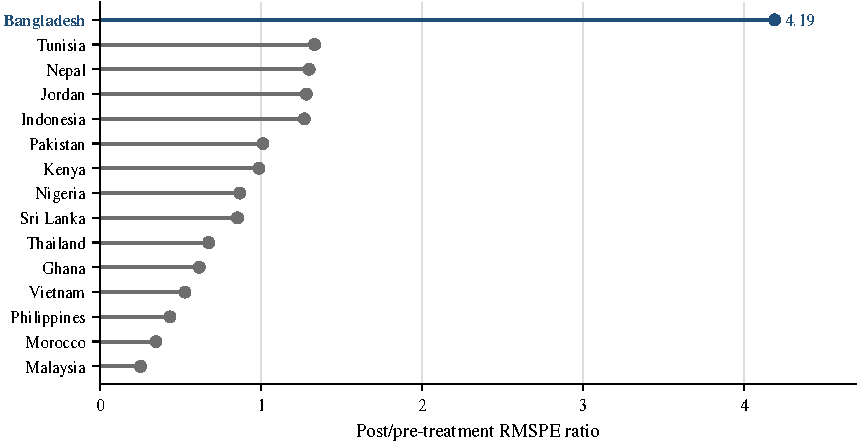
\includegraphics[width=\textwidth]{fig2_sc_placebo_rmspe_ratio.pdf}
\fignote{Each donor country is assigned the July 18--23 treatment in turn, and its synthetic control is rebuilt from the remaining donors. The figure ranks Bangladesh and the 14 placebo countries by the ratio of post-treatment to pre-treatment RMSPE, a statistic that scales the treatment-period gap by each unit's pre-treatment fit. Bangladesh is the most extreme of the 15 units; it also has the largest absolute ATT. The exact rank $p$-value is therefore $1/15 = 0.0667$ for both statistics. This is the minimum attainable value with 14 placebo countries: Bangladesh is the most extreme unit in the placebo distribution, but the resolution of exact placebo inference is limited by the size of the donor pool. Source: \texttt{results/synthetic\_control/sc\_inspace\_placebos.csv}, verified against \texttt{results/final/table\_primary\_SC\_placebos.csv}.}
\end{figure}

The leave-one-out exercise is highly stable (\cref{tab:loo} in \cref{sec:sc_diagnostics}). Across specifications that remove one donor at a time, the ATT ranges only from $-$13.256 to $-$12.886 percentage points. In particular, excluding Pakistan produces $-$12.905 percentage points, excluding Ghana produces $-$13.209 percentage points, and excluding Kenya produces $-$12.886 percentage points. This matters because both Pakistan and Kenya experienced localized connectivity disruptions near the broader pre-treatment period: Internet Society reports regional restrictions in Pakistan around July 14--17, while Cloudflare documents a major Kenyan traffic disruption on June 25 \citep{isoc2024,cloudflare2024}.
% TODO: REPLACE BANGLADESH INTERNET SOCIETY ENTRY WITH PAKISTAN-SPECIFIC SOURCE
The limited movement in the treatment estimate when either donor is removed reduces, though does not eliminate, concern that these donor-specific episodes drive the result.

\subsection{Difference-in-differences and event study}
\label{sec:did_results}

The international DiD estimate is $-$13.088 percentage points, nearly identical to the synthetic-control ATT (\cref{tab:did}, Panel A). Removing national holidays yields $-$13.379 percentage points. The agreement is notable because the two methods use different weighting logic: synthetic control chooses donor weights to reproduce Bangladesh before the shutdown, whereas the international DiD gives equal weight to donor-country changes. Bangladesh's estimate is also more extreme than that of every in-space placebo, whose estimates range from $-$1.72 to 1.60 percentage points; as for the synthetic control, the resulting rank value of 0.0667 is the minimum attainable with fifteen countries.

% Generated by analysis/tables/make_all_tables.py -- do not edit by hand.
\begin{table}[htbp]
\centering
\footnotesize
\caption{International difference-in-differences and aggregate event study}
\label{tab:did}
\begin{threeparttable}
\begin{tabular}{lrrrrrrr}
\toprule
& BD pre & BD shut- & Donor & ATT & Relative & Placebo & Rank \\
Specification & (\%) & down (\%) & change & (pp) & effect & SD & $p$ \\
\midrule
\multicolumn{8}{l}{\textit{A. Difference-in-differences, July 18--23 vs.\ May 1--July 17}} \\
All days & 17.25 & 2.02 & $-$2.15 & $-$13.09 & $-$86.6\% & 1.17 & 0.0667 \\
Holidays excluded & 17.58 & 2.02 & $-$2.18 & $-$13.38 & $-$86.9\% & 1.19 & 0.0667 \\
\addlinespace \multicolumn{8}{l}{\textit{B. Event study, selected weeks (all weeks in \cref{tab:did_es_full})}} \\
\multicolumn{4}{l}{Event week (dates)} & $\hat\theta_k$ (pp) & Placebo-based interval & Placebo SD & Rank $p$ \\
\multicolumn{4}{l}{$-5$ (Jun 13--Jun 19)} & $-$4.89 & [$-$9.31, $-$0.47] & 2.26 & 0.0667 \\
\multicolumn{4}{l}{$-2$ (Jul 4--Jul 10)} & 6.10 & [3.76, 8.43] & 1.19 & 0.0667 \\
\multicolumn{4}{l}{$-1$ (Jul 11--Jul 17)} & 3.86 & [2.15, 5.58] & 0.88 & 0.0667 \\
\multicolumn{4}{l}{$0$ (Jul 18--Jul 23)} & $-$13.09 & [$-$15.39, $-$10.79] & 1.17 & 0.0667 \\
\multicolumn{4}{l}{$+1$ (Jul 24--Jul 30)} & $-$2.66 & [$-$5.35, 0.02] & 1.37 & 0.0667 \\
\multicolumn{4}{l}{$+2$ (Jul 31--Aug 6)} & $-$2.76 & [$-$4.87, $-$0.65] & 1.08 & 0.0667 \\
\multicolumn{4}{l}{$+3$ (Aug 7--Aug 13)} & 0.52 & [$-$1.99, 3.02] & 1.28 & 0.9333 \\
\multicolumn{4}{l}{$+4$ (Aug 14--Aug 20)} & 4.31 & [1.99, 6.64] & 1.18 & 0.0667 \\
\multicolumn{4}{l}{$+5$ (Aug 21--Aug 27)} & 4.84 & [2.40, 7.28] & 1.24 & 0.0667 \\
\multicolumn{4}{l}{$+6$ (Aug 28--Sep 3)} & 2.53 & [0.01, 5.05] & 1.29 & 0.0667 \\
\bottomrule
\end{tabular}
\begin{tablenotes}[flushleft]
\footnotesize\raggedright
\item \textit{Notes:} Outcome: daily percentage of eligible users with observable productive GitHub activity. Panel A compares Bangladesh's change from May 1--July 17 to July 18--23 with the equal-weighted mean change of the 14 donor countries (\cref{eq:did_agg}); the ATT reproduces \texttt{results/final/table\_DiD\_all\_outcomes.csv}. Panel B reports $\hat\theta_k$ (\cref{eq:es_agg}) for weekly bins; week 0 equals the Panel A all-days ATT. Weeks $-5$ and $-2$ are the most negative and most positive pre-shutdown estimates. Inference uses in-space placebos: each donor is compared in turn with the mean of the other 13. \textit{Placebo SD}: standard deviation of the 14 placebo estimates. \textit{Placebo-based interval}: $\hat\theta_k\pm1.96\times$SD, a donor-placebo reference interval, not a conventional sampling confidence interval. \textit{Rank $p$}: share of the 15 units whose absolute estimate is at least as large as Bangladesh's (minimum 0.0667). Bangladesh's pre-period weekly estimates are more volatile than any donor's, so these placebo-based measures are not fully calibrated sampling uncertainty for Bangladesh. The pre-period does not show a clean parallel-trends pattern, and the weekly coefficients are a diagnostic, not an identified dynamic treatment path; the synthetic control remains the main design. Sources: \texttt{results/did/did\_main\_placebo\_inference.csv}, \texttt{results/did/did\_eventstudy\_weekly.csv}.
\end{tablenotes}
\end{threeparttable}
\end{table}


\Cref{fig:did_es} reports the weekly event study from \cref{eq:es_agg}. Its shutdown-week coefficient, $-$13.09 percentage points, reproduces the aggregate DiD estimate and is more than twice as large in absolute value as any pre-shutdown weekly coefficient. The pre-shutdown period, however, is volatile and does not display a clean conventional parallel-trends pattern. Weekly coefficients range from $-$4.89 percentage points (week $-5$, June 13--19) to 6.10 (week $-2$, July 4--10), and Bangladesh was above its pre-period position relative to the donors in the two weeks immediately before the shutdown. This mirrors the imperfect early-July fit of the synthetic control (\cref{fig:sc}). Because the reference is the full pre-period mean, this elevated activity does not generate the shutdown estimate; measured against the immediately preceding week alone, the decline would be larger. Given this pre-period volatility, the weekly coefficients are not interpreted as an identified dynamic causal treatment path. They are diagnostic evidence that the largest break in the series is concentrated in the shutdown week.

\begin{figure}[htbp]
\centering
\caption{Diagnostic event study: Bangladesh relative to the equal-weighted donor mean, by week}
\label{fig:did_es}
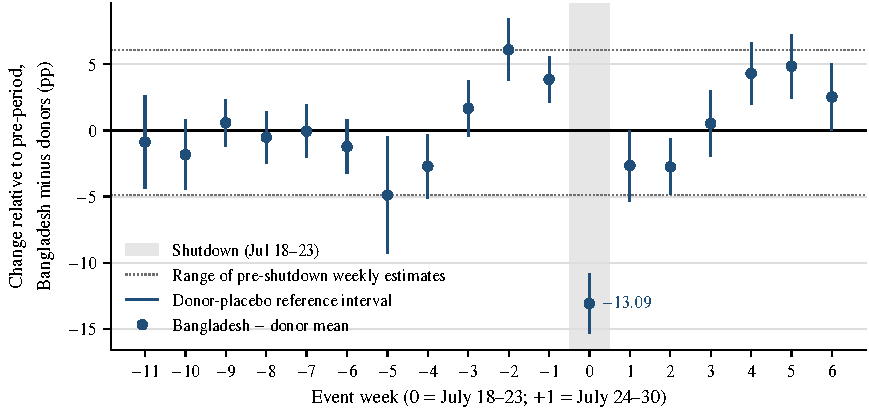
\includegraphics[width=\textwidth]{fig3_did_eventstudy.pdf}
\fignote{Points are $\hat\theta_k$ from \cref{eq:es_agg}: the change in Bangladesh's daily percentage of eligible users with observable productive GitHub activity, relative to its May 1--July 17 mean, minus the corresponding change averaged over the 14 donor countries with equal weights. Week 0 is the July 18--23 shutdown (shaded); its coefficient equals the DiD estimate in \cref{tab:did}. Weeks $-11$ to $-1$ are seven-day bins ending July 17 (week $-11$ includes May 1); weeks $+1$ to $+6$ are seven-day bins from July 24 to September 3. Vertical lines are donor-placebo reference intervals, $\hat\theta_k \pm 1.96$ times the standard deviation of the 14 in-space placebo estimates for the same week; they are not conventional sampling confidence intervals. Dotted horizontal lines mark the minimum and maximum of Bangladesh's pre-shutdown weekly coefficients. Bangladesh's pre-period estimates are more volatile than those of any donor country, so the reference intervals should not be interpreted as fully calibrated sampling uncertainty. The pre-period does not show a clean parallel-trends pattern; the coefficients are a diagnostic complement to the synthetic control, not an identified dynamic treatment path. Source: \texttt{results/did/did\_eventstudy\_weekly.csv} (script \texttt{analysis/did/01\_aggregate\_did\_eventstudy.py}, input \texttt{results/synthetic\_control/country\_day\_donor\_pool\_with\_holidays.parquet}). Week 0 is verified against \texttt{results/final/table\_DiD\_all\_outcomes.csv}.}
\end{figure}

The donor-placebo reference intervals in \cref{fig:did_es} should be read with care. They are not conventional sampling confidence intervals: they scale the spread of the fourteen donor placebo estimates in each week. Bangladesh's pre-shutdown weekly coefficients have a standard deviation of 3.04 percentage points, compared with 0.70 to 2.18 percentage points for the donors treated as placebo units. Several pre-period coefficients for Bangladesh are therefore as extreme as any placebo, and the reference intervals are not fully calibrated measures of uncertainty for Bangladesh. The more informative comparison is with Bangladesh's own pre-shutdown range: the shutdown coefficient lies far outside it, whereas every post-restoration coefficient lies within it.

After restoration, the gap narrows quickly. The coefficients are $-$2.66 and $-$2.76 percentage points in the two weeks after the shutdown and are positive from week $+3$ onward. The positive coefficients in weeks $+4$ to $+6$ (2.53 to 4.84 percentage points) lie within the range of pre-shutdown fluctuations and should not be interpreted as gains caused by the shutdown. User-day event-study estimates from earlier auxiliary analyses are not reported because their implementation is not fully documented. Recovery dynamics within Bangladesh are examined by repository sector in \cref{sec:sector_results}.

\subsection{Regression discontinuity in time}
\label{sec:rdit_results}

\Cref{fig:rdit} shows the daily series used in the RDiT. In Bangladesh, the share of users with productive activity is 19.03 percent on July 17, falls to 10.74 percent on July 18, and lies between 0.48 and 1.23 percent from July 19 through July 23 before recovering gradually from July 24. The Philippines, used as a geographic placebo, shows no comparable break.

\begin{figure}[htbp]
\centering
\caption{Regression discontinuity in time: daily share of users with productive activity around the July 17 cutoff (visual companion to \cref{tab:rdit})}
\label{fig:rdit}
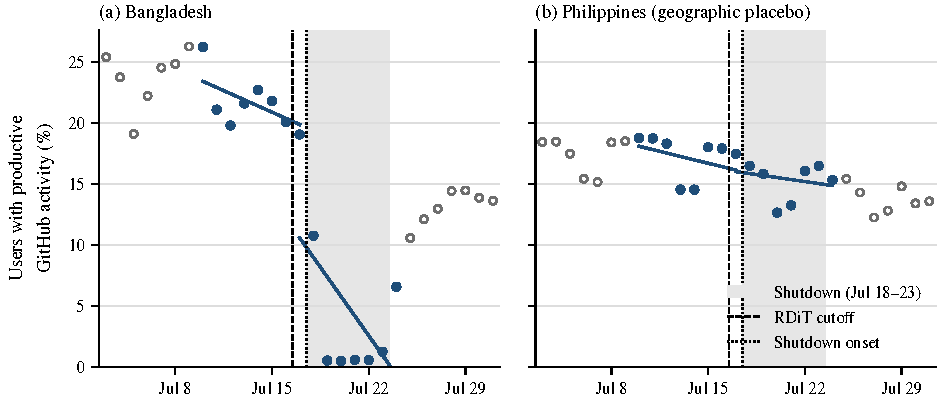
\includegraphics[width=\textwidth]{fig7_rdit_cutoff.pdf}
\fignote{Daily percentage of users with at least one productive GitHub event in the balanced user-day panels used for the RDiT (10,329 Bangladesh-associated and 3,025 Philippines-associated accounts), July 3--31, 2024. Filled markers are the fifteen days inside the 7-day bandwidth of \cref{eq:rdit} (July 10--24); hollow markers are shown for context. Lines are the local linear fits of the archived preferred specification on each side of the cutoff; the dashed vertical line marks the RDiT cutoff, with July 17 ($\tilde t=0$) on the post-cutoff side, and the dotted vertical line marks the shutdown boundary between July 17 and July 18. The shaded band is the July 18--23 shutdown. The figure is a visual companion to the formal estimates in \cref{tab:rdit}; the fitted lines correspond exactly to those estimates. Source: \texttt{results/rdit/rdit\_daily\_series.csv}, written by \texttt{analysis/rdit/01\_reproduce\_rdit.py} from \texttt{data/processed/panel\_user\_day\_bangladesh.parquet} and \texttt{panel\_user\_day\_philippines.parquet}; the same script reproduces the archived estimates in \texttt{results/rdit/main\_rdit\_summary.csv} exactly.}
\end{figure}

The RDiT produces a smaller point estimate but the same qualitative conclusion (\cref{tab:rdit}). The preferred local linear specification estimates a discontinuity of $-$9.28 percentage points in Bangladesh's active-user rate; a controlled Bangladesh-minus-Philippines version yields $-$9.16 percentage points. HAC $p$-values are approximately 0.065 in both cases, while the Philippines placebo is near zero. The smaller magnitude than in the synthetic control and DiD is consistent with the design visible in \cref{fig:rdit}: the cutoff day, July 17, precedes the shutdown but lies on the post-cutoff side, and the linear post-cutoff fit spans both the collapse and the beginning of the recovery on July 24.
Consistent with \citet{hausman2018}, I therefore emphasize the direction and timing of the break rather than treating the RDiT $p$-value as the decisive inferential statistic.

% Generated by analysis/tables/make_all_tables.py -- do not edit by hand.
\begin{table}[H]
\centering
\footnotesize
\caption{Regression discontinuity in time: preferred specification}
\label{tab:rdit}
\begin{threeparttable}
\begin{tabular}{l>{\raggedright\arraybackslash}p{3.3cm}rrcrr}
\toprule
Specification & Outcome & Effect (pp) & HAC SE & 95\% CI & $p$ & Days \\
\midrule
Main local linear & Bangladesh active rate & $-$9.284 & 5.034 & [$-$19.151, 0.584] & 0.065 & 15 \\
Controlled local linear & Bangladesh $-$ Philippines active rate & $-$9.160 & 4.980 & [$-$18.921, 0.601] & 0.066 & 15 \\
Geographic placebo & Philippines active rate & $-$0.124 & 1.492 & [$-$3.048, 2.801] & 0.934 & 15 \\
\bottomrule
\end{tabular}
\begin{tablenotes}[flushleft]
\footnotesize\raggedright
\item \textit{Notes:} Local linear RDiT at the July 17, 2024 cutoff, bandwidth 7 days, polynomial degree 1, no donut, HAC lags 2. Effects are reported in percentage points. RDiT is a temporal robustness check, not the primary causal design. Source: \texttt{results/rdit/main\_rdit\_summary.csv}.
\end{tablenotes}
\end{threeparttable}
\end{table}


\subsection{Productive, shipping, and collaboration outcomes}
\label{sec:secondary}

The collapse is not limited to a generic activity indicator. Holding the primary synthetic-control weights fixed, productive activity falls by 15.179 percentage points relative to a 17.555 percent counterfactual, or 86.5 percent. Shipping activity falls by 1.333 percentage points relative to a 1.415 percent counterfactual, or 94.2 percent. Collaboration activity falls by 0.780 percentage points relative to a 0.834 percent counterfactual, or 93.6 percent. Count outcomes show similarly large relative declines in collaboration events and shipping output (\cref{tab:secondary}). International DiD estimates for the same outcomes, which point in the same direction, are reported in \cref{tab:did_secondary}.

Allowing the donor weights to re-optimize separately for each outcome produces comparable magnitudes: $-$86.2 percent for productive activity, $-$92.2 percent for shipping activity, and $-$92.1 percent for collaboration activity. The in-space placebo ATT rank is again 0.0667 for all three key activity-rate outcomes. The RMSPE-ratio rank is 0.0667 for productive and shipping activity but 0.20 for collaboration activity. I therefore treat collaboration as consistent secondary evidence rather than giving it the same inferential weight as the primary and shipping outcomes.

% Generated by analysis/tables/make_all_tables.py -- do not edit by hand.
\begin{table}[htbp]
\centering
\footnotesize
\caption{Secondary outcomes}
\label{tab:secondary}
\begin{threeparttable}
\begin{tabular}{lrrrrrr}
\toprule
 & \multicolumn{2}{c}{Fixed primary weights} & \multicolumn{2}{c}{Outcome-specific weights} & \multicolumn{2}{c}{Placebo rank} \\ \cmidrule(lr){2-3}\cmidrule(lr){4-5}\cmidrule(lr){6-7}
Outcome & ATT & Relative & ATT & Relative & ATT & RMSPE ratio \\
\midrule
Productive active rate & $-$15.179 pp & $-$86.5\% & $-$14.870 pp & $-$86.2\% & 0.0667 & 0.0667 \\
Shipping active rate & $-$1.333 pp & $-$94.2\% & $-$0.964 pp & $-$92.2\% & 0.0667 & 0.0667 \\
Collaboration active rate & $-$0.780 pp & $-$93.6\% & $-$0.630 pp & $-$92.1\% & 0.0667 & 0.2000 \\
Collaboration events / 1,000 & $-$24.095 & $-$95.1\% & $-$18.589 & $-$93.7\% & -- & -- \\
Shipping output / 1,000 & $-$23.981 & $-$93.9\% & $-$18.192 & $-$92.1\% & -- & -- \\
\bottomrule
\end{tabular}
\begin{tablenotes}[flushleft]
\footnotesize\raggedright
\item \textit{Notes:} Fixed-weight specifications reuse the primary active-rate SCM weights (\cref{tab:weights}). Outcome-specific specifications re-estimate donor weights separately for each outcome (\cref{tab:weights_specific}). Rank values are exact in-space placebo ranks for the outcome-specific specifications with 14 placebo countries; 0.0667 is the minimum attainable value. Placebo ranks are not reported for the count outcomes.
\end{tablenotes}
\end{threeparttable}
\end{table}


\subsection{Sectoral recovery after restoration}
\label{sec:sector_results}

The synthetic-control estimates describe the collapse during the shutdown window. They do not show how activity evolved once connectivity returned, or whether recovery was common across the kinds of projects on which Bangladeshi developers work. This subsection addresses these questions using the fixed sample of 20,000 Bangladesh-associated accounts and the repository-sector classification of \cref{sec:sector_data}, estimated as described in \cref{sec:sector_method}. The analysis compares each sector with its own pre-shutdown baseline. It documents heterogeneity in recovery dynamics within Bangladesh; it does not estimate sector-specific causal effects relative to an untreated international control, and the synthetic-control estimate in \cref{sec:main_results} remains the paper's headline result. Throughout, a sector refers to the economic sector associated with the repositories in which observable GitHub activity occurs, not to developers' employers or industries of employment.

% Generated by analysis/tables/make_all_tables.py -- do not edit by hand.
\begin{table}[htbp]
\centering
\footnotesize
\caption{Recovery of observable GitHub push activity by repository sector}
\label{tab:sector_recovery}
\begin{threeparttable}
\begin{tabular}{lrrrrrrrrr}
\toprule
& & Pre & Pre rate & \multicolumn{5}{c}{Recovery index (pre-period mean = 100)} & First wk \\
\cmidrule(lr){5-9}
Sector & NAICS & users & (\%) & Shutdown & +1 & +2 & +4 & +8 & $\geq$80, 2 wks \\
\midrule
Finance & 52 & 382 & 0.078 & 30.9 & 92.2 & 67.6 & 89.5 & 91.3 & 3 \\
Information & 51 & 1,528 & 0.442 & 11.7 & 75.9 & 72.2 & 106.0 & 94.5 & 3 \\
Education & 61 & 1,234 & 0.385 & 11.7 & 59.1 & 53.4 & 75.4 & 81.9 & 6 \\
Health & 62 & 514 & 0.132 & 6.3 & 40.7 & 51.5 & 77.5 & 89.4 & 6 \\
Retail & 44--45 & 1,012 & 0.295 & 6.2 & 52.0 & 52.3 & 153.7 & 79.6 & 9 \\
Real Estate & 53 & 213 & 0.063 & 4.0 & 33.0 & 25.1 & 44.4 & 85.5 & 5 \\
Accommodation/Food & 72 & 480 & 0.144 & 3.5 & 44.3 & 42.8 & 54.2 & 62.6 & -- \\
\bottomrule
\end{tabular}
\begin{tablenotes}[flushleft]
\footnotesize\raggedright
\item \textit{Notes:} Fixed sample of 20,000 Bangladesh-associated accounts. Repository sectors from the historical-README classifier with confidence $\geq$ 0.80. The outcome is the share of sampled users with at least one PushEvent to a repository of the sector on a given day. \textit{Pre users}: sampled users with such activity in the baseline period. \textit{Pre rate}: mean daily outcome over the baseline period (May 23--July 17, 2024, the final eight complete pre-shutdown weeks), in percent of all 20,000 users. Shutdown: July 18--23; week +1: July 24--30; subsequent 7-day bins. \textit{First wk $\geq$80, 2 wks}: first post-shutdown week that begins two consecutive weeks with an index of at least 80 (observed through week +17, November 13--19); it does not imply that the index stays above 80 thereafter. -- indicates no such week. Within-Bangladesh comparison with the sector's own pre-period; not a causal effect relative to an untreated control. Sources: \texttt{results/sector\_recovery/sectorwide/sectorwide\_recovery\_summary.csv}, verified against \texttt{results/sector\_recovery/final/table\_sector\_recovery\_main.csv}.
\end{tablenotes}
\end{threeparttable}
\end{table}


All seven sectors show a sharp fall in observable push activity during July 18--23 (\cref{tab:sector_recovery,fig:sector_index}). The shutdown-period recovery index ranges from 3.5 in Accommodation/Food to 11.7 in Information and Education and 30.9 in Finance. In every sector, the 95 percent confidence interval for the change relative to the baseline excludes zero (\cref{fig:sector_es}).

Restoration of connectivity did not imply an immediate or uniform recovery. In the first week after the shutdown (July 24--30), the recovery index ranges from 33.0 in Real Estate to 92.2 in Finance. Mobile connectivity returned only during this week, later than fixed broadband \citep{belson2024}, so part of the week $+1$ shortfall may reflect incomplete restoration. Recovery was also not monotonic: in Finance, Information, Education, Real Estate, and Accommodation/Food, the index is lower in week $+2$ (July 31--August 6) than in week $+1$. The data do not identify the source of this second-week decline.

\begin{figure}[htbp]
\centering
\caption{Recovery of observable GitHub push activity by repository sector}
\label{fig:sector_index}
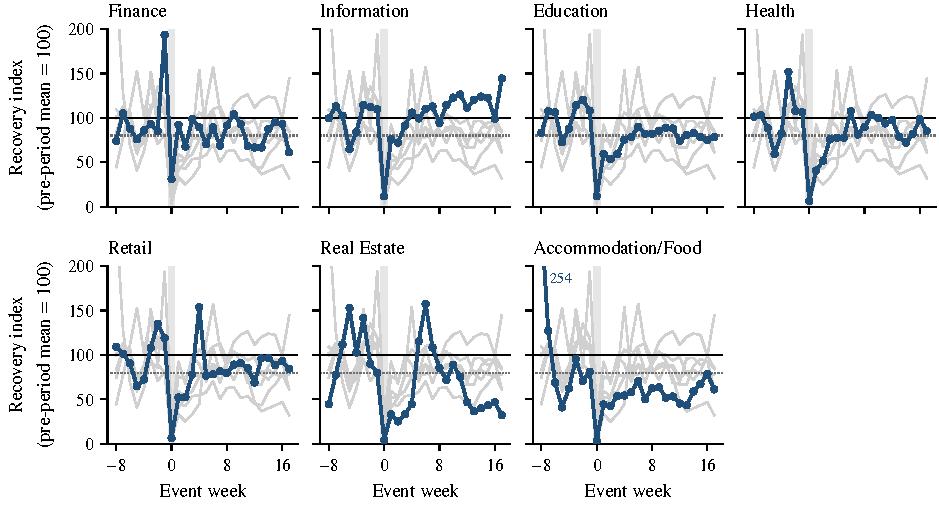
\includegraphics[width=\textwidth]{fig5_sector_recovery_index.pdf}
\fignote{Each panel highlights one sector's recovery index $R_{sk}$ (\cref{eq:sector}); the other six sectors are shown in light grey for comparison. The index is 100 times the sector's mean daily probability of push activity in event week $k$, divided by its mean over the final eight complete pre-shutdown weeks (May 23--July 17, 2024). The shaded band is the July 18--23 shutdown ($k=0$); week $+1$ is July 24--30, followed by consecutive seven-day bins. Solid and dotted horizontal lines mark 100 and 80. The common vertical axis is truncated at 200; the one value above it (Accommodation/Food, week $-8$) is labeled. Fixed sample of 20,000 Bangladesh-associated accounts; repository sectors from the historical-README classifier with confidence $\geq 0.80$. The sector is that of the repositories in which activity occurs, not the developer's employer. Within-Bangladesh comparison with each sector's own baseline; not a causal effect relative to an untreated control. Source: \texttt{results/sector\_recovery/sectorwide/sectorwide\_user\_eventstudy.csv}, verified against \texttt{results/sector\_recovery/final/table\_sector\_recovery\_main.csv}.}
\end{figure}

Finance and Information recovered fastest. Finance returned to an index of 92.2 in week $+1$, and both sectors begin a run of two consecutive weeks at or above 80 in week $+3$. Information exceeds its baseline by week $+4$ (106.0). In week $+8$, the two indices are 94.5 and 91.3. The Finance series is nonetheless noisy: its baseline includes a spike in week $-1$ (index 193.6), and its post-shutdown index falls back below 80 in several later weeks.

Education and Health recovered more gradually. Their week $+1$ indices are 59.1 and 40.7, they reach 75.4 and 77.5 by week $+4$, and both begin a run of two consecutive weeks at or above 80 only in week $+6$. By week $+8$, they stand at 81.9 and 89.4.

Accommodation/Food remained persistently depressed. Its index is 44.3 in week $+1$, 54.2 in week $+4$, and 62.6 in week $+8$, and it never records two consecutive weeks at or above 80 through the end of the observation window (week $+17$, November 13--19). This result should be read alongside the sector's unstable baseline: the index is 254.1 and 127.3 in the first two baseline weeks and between 40.8 and 95.5 in the remaining six. Part of the post-shutdown gap may therefore reflect a decline that began before the shutdown rather than a failure to recover.

Real Estate recovered slowly at first and later approached its baseline. Its index remains between 25.1 and 44.4 through week $+4$, rises above 100 in weeks $+5$ and $+6$ (115.1 and 157.3), and is 85.5 in week $+8$. This later recovery is not durable within the observed window: from week $+12$ onward, the index lies between 31.9 and 46.7 (\cref{fig:sector_es}). Real Estate is also the smallest of the seven sectors, with 213 sampled users active in the baseline period, so its weekly estimates are imprecise.

Retail shows a pronounced temporary rebound. Its index is about 52 in weeks $+1$ and $+2$, rises to 153.7 in week $+4$ (August 14--20), and falls back to 76.5 in week $+5$. Its first run of two consecutive weeks at or above 80 begins only in week $+9$. The week $+4$ value is therefore a transient overshoot, possibly reflecting a burst of catch-up activity, rather than evidence of completed recovery; the data do not identify what generated it. The timing of Retail's first sustained run is also sensitive to the classifier threshold (\cref{sec:sector_robustness}).

Index values above 100 later in the window should not be read as gains caused by the shutdown. Information, for example, has an index between 111.5 and 126.4 in weeks $+10$ to $+15$ and 144.3 in week $+17$. Without an untreated comparison group, such movements cannot be separated from trend growth, seasonality, or changes in the sampled users' activity.

\begin{figure}[htbp]
\centering
\caption{Sectoral event study: change in daily push-activity probability relative to the pre-shutdown baseline}
\label{fig:sector_es}
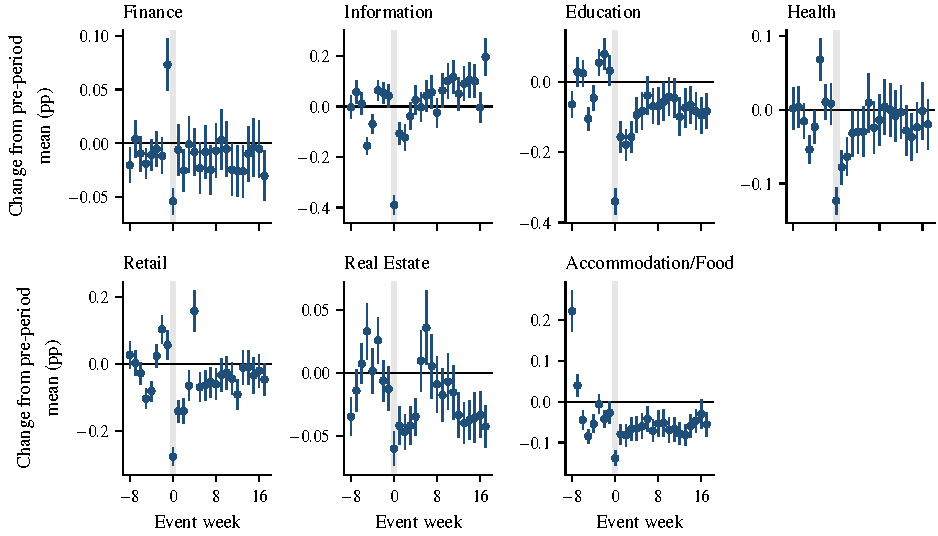
\includegraphics[width=\textwidth]{fig6_sector_eventstudy.pdf}
\fignote{Points are $\beta_{sk}$ from \cref{eq:sector}: the mean change, across the fixed sample of 20,000 Bangladesh-associated accounts, in the daily probability of a PushEvent in a sector-$s$ repository during event week $k$, relative to each user's mean over the final eight complete pre-shutdown weeks, in percentage points. Vertical lines are 95 percent confidence intervals based on the cross-user standard deviation of these differences; they do not account for common weekly shocks. The shaded band is the July 18--23 shutdown ($k=0$); week $+1$ is July 24--30, and the window extends to week $+17$ (November 13--19, 2024). Vertical scales differ across panels because baseline activity levels differ by sector (\cref{tab:sector_recovery}). Repository sectors from the historical-README classifier with confidence $\geq 0.80$. Within-Bangladesh comparison; not a causal effect relative to an untreated control. Source: \texttt{results/sector\_recovery/sectorwide/sectorwide\_user\_eventstudy.csv}.}
\end{figure}

The main specification counts pushes to any classified repository, including repositories first observed after the shutdown. A complementary specification follows only repositories pushed to during the eight baseline weeks (\cref{tab:sector_fixed_repo}). Activity in these pre-existing repositories recovers far less: in week $+8$, their indices range from 10.1 (Accommodation/Food) to 31.4 (Education), compared with 62.6 to 94.5 in the sector-wide specification. Because repositories selected on recent activity would become less active over time even without a shutdown, this gap does not measure a shutdown effect. It is nevertheless consistent with recovery occurring partly through new repositories and switching across projects rather than solely through a return to pre-existing ones.

Taken together, the sectoral evidence indicates that the collapse in observable activity documented in \cref{sec:main_results} was followed by a recovery that was gradual and uneven across the economic sectors associated with developers' repositories. These are before--after comparisons within Bangladesh. They share the identification limitations discussed in \cref{sec:unrest} and, in addition, cannot separate post-shutdown recovery from other Bangladesh-specific developments between August and November 2024.
